% Options for packages loaded elsewhere
\PassOptionsToPackage{unicode}{hyperref}
\PassOptionsToPackage{hyphens}{url}
%
\documentclass[
  ignorenonframetext,
]{beamer}
\usepackage{pgfpages}
\setbeamertemplate{caption}[numbered]
\setbeamertemplate{caption label separator}{: }
\setbeamercolor{caption name}{fg=normal text.fg}
\beamertemplatenavigationsymbolsempty
% Prevent slide breaks in the middle of a paragraph
\widowpenalties 1 10000
\raggedbottom
\setbeamertemplate{part page}{
  \centering
  \begin{beamercolorbox}[sep=16pt,center]{part title}
    \usebeamerfont{part title}\insertpart\par
  \end{beamercolorbox}
}
\setbeamertemplate{section page}{
  \centering
  \begin{beamercolorbox}[sep=12pt,center]{part title}
    \usebeamerfont{section title}\insertsection\par
  \end{beamercolorbox}
}
\setbeamertemplate{subsection page}{
  \centering
  \begin{beamercolorbox}[sep=8pt,center]{part title}
    \usebeamerfont{subsection title}\insertsubsection\par
  \end{beamercolorbox}
}
\AtBeginPart{
  \frame{\partpage}
}
\AtBeginSection{
  \ifbibliography
  \else
    \frame{\sectionpage}
  \fi
}
\AtBeginSubsection{
  \frame{\subsectionpage}
}
\usepackage{amsmath,amssymb}
\usepackage{lmodern}
\usepackage{ifxetex,ifluatex}
\ifnum 0\ifxetex 1\fi\ifluatex 1\fi=0 % if pdftex
  \usepackage[T1]{fontenc}
  \usepackage[utf8]{inputenc}
  \usepackage{textcomp} % provide euro and other symbols
\else % if luatex or xetex
  \usepackage{unicode-math}
  \defaultfontfeatures{Scale=MatchLowercase}
  \defaultfontfeatures[\rmfamily]{Ligatures=TeX,Scale=1}
\fi
\usetheme[]{Frankfurt}
% Use upquote if available, for straight quotes in verbatim environments
\IfFileExists{upquote.sty}{\usepackage{upquote}}{}
\IfFileExists{microtype.sty}{% use microtype if available
  \usepackage[]{microtype}
  \UseMicrotypeSet[protrusion]{basicmath} % disable protrusion for tt fonts
}{}
\makeatletter
\@ifundefined{KOMAClassName}{% if non-KOMA class
  \IfFileExists{parskip.sty}{%
    \usepackage{parskip}
  }{% else
    \setlength{\parindent}{0pt}
    \setlength{\parskip}{6pt plus 2pt minus 1pt}}
}{% if KOMA class
  \KOMAoptions{parskip=half}}
\makeatother
\usepackage{xcolor}
\IfFileExists{xurl.sty}{\usepackage{xurl}}{} % add URL line breaks if available
\IfFileExists{bookmark.sty}{\usepackage{bookmark}}{\usepackage{hyperref}}
\hypersetup{
  pdftitle={Hypodermic needle after all? Individual-level Moderators of Media Framing Effects},
  pdfauthor={Nicolai Berk\^{}*},
  hidelinks,
  pdfcreator={LaTeX via pandoc}}
\urlstyle{same} % disable monospaced font for URLs
\newif\ifbibliography
\usepackage{graphicx}
\makeatletter
\def\maxwidth{\ifdim\Gin@nat@width>\linewidth\linewidth\else\Gin@nat@width\fi}
\def\maxheight{\ifdim\Gin@nat@height>\textheight\textheight\else\Gin@nat@height\fi}
\makeatother
% Scale images if necessary, so that they will not overflow the page
% margins by default, and it is still possible to overwrite the defaults
% using explicit options in \includegraphics[width, height, ...]{}
\setkeys{Gin}{width=\maxwidth,height=\maxheight,keepaspectratio}
% Set default figure placement to htbp
\makeatletter
\def\fps@figure{htbp}
\makeatother
\setlength{\emergencystretch}{3em} % prevent overfull lines
\providecommand{\tightlist}{%
  \setlength{\itemsep}{0pt}\setlength{\parskip}{0pt}}
\setcounter{secnumdepth}{-\maxdimen} % remove section numbering

\ifluatex
  \usepackage{selnolig}  % disable illegal ligatures
\fi
\newlength{\cslhangindent}
\setlength{\cslhangindent}{1.5em}
\newlength{\csllabelwidth}
\setlength{\csllabelwidth}{3em}
\newenvironment{CSLReferences}[2] % #1 hanging-ident, #2 entry spacing
 {% don't indent paragraphs
  \setlength{\parindent}{0pt}
  % turn on hanging indent if param 1 is 1
  \ifodd #1 \everypar{\setlength{\hangindent}{\cslhangindent}}\ignorespaces\fi
  % set entry spacing
  \ifnum #2 > 0
  \setlength{\parskip}{#2\baselineskip}
  \fi
 }%
 {}
\usepackage{calc}
\newcommand{\CSLBlock}[1]{#1\hfill\break}
\newcommand{\CSLLeftMargin}[1]{\parbox[t]{\csllabelwidth}{#1}}
\newcommand{\CSLRightInline}[1]{\parbox[t]{\linewidth - \csllabelwidth}{#1}\break}
\newcommand{\CSLIndent}[1]{\hspace{\cslhangindent}#1}

\title{Hypodermic needle after all? Individual-level Moderators of Media
Framing Effects}
\subtitle{Presentation at EPSIP Colloquium, HU Berlin}
\author{Nicolai Berk\(^*\)}
\date{May 3rd, 2021}
\institute{\(^*\)RTG Dynamics/Humboldt Universität zu Berlin}

\begin{document}
\frame{\titlepage}

\hypertarget{motivation}{%
\section{Motivation}\label{motivation}}

\hypertarget{media-effects---maximal-or-minimal}{%
\subsection{Media effects - maximal or
minimal?}\label{media-effects---maximal-or-minimal}}

\begin{frame}[allowframebreaks]{Media effects - maximal or minimal?}
\center

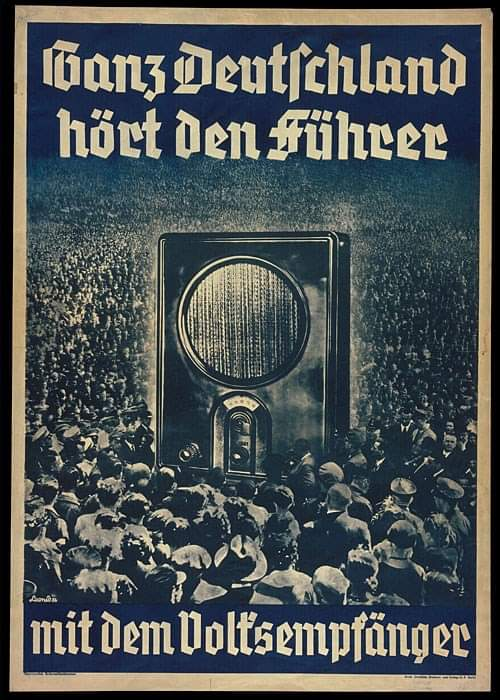
\includegraphics[width=0.4\textwidth,height=\textheight]{vis/volksempfanger.jpg}
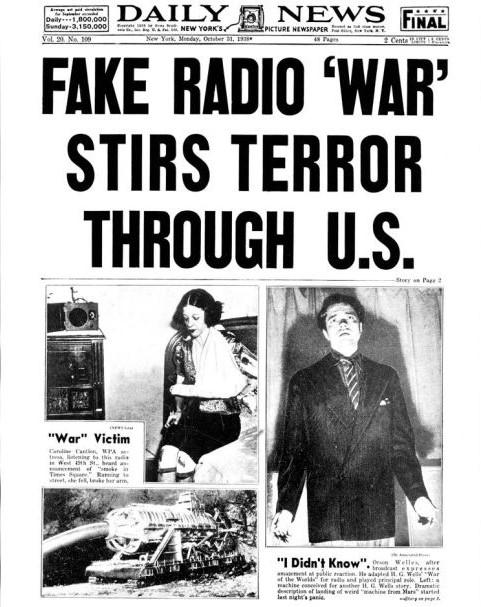
\includegraphics[width=0.4\textwidth,height=\textheight]{vis/ufo_scares.jpg}

\flushleft

\framebreak

Maximal paradigm also follows from classic work

\begin{itemize}
\tightlist
\item
  attitude instability (Converse 1962; Zaller 1992)
\item
  framing (Nelson, Clawson, and Oxley 1997)
\item
  agenda-setting (McCombs and Shaw 1972)
\end{itemize}

\framebreak

\center


\includegraphics[width=0.3\textwidth,height=\textheight]{vis/mineff.png}

\flushleft

Minimal effects assumption with increasing media diversity (Bennett and
Iyengar 2008):

\begin{itemize}
\tightlist
\item
  media environment more polarised and more diverse,
\item
  viewers more likely to reject news conflicting with their views,
\item
  viewers can opt for other sources.
\end{itemize}

\(\rightarrow\) strong effects unlikely

\framebreak

Evidence seems to support both views:
\end{frame}

\begin{frame}{strong media effects on:}
\protect\hypertarget{strong-media-effects-on}{}
\begin{itemize}
\tightlist
\item
  voting behaviour (Boomgaarden and Vliegenthart 2009; Devine and Murphy
  2020; Ladd and Lenz 2009),
\item
  issue agenda (King, Schneer, and White 2017),
\item
  attitudes (Nelson, Clawson, and Oxley 1997; Foos and Bischof 2020)
\end{itemize}
\end{frame}

\begin{frame}{weak or no effects on:}
\protect\hypertarget{weak-or-no-effects-on}{}
\begin{itemize}
\tightlist
\item
  voting behaviour (Gentzkow, Shapiro, and Sinkinson 2011),
\item
  issue agenda (Lau, Rogers, and Love 2021),
\item
  attitudes (Guess et al. 2021).
\end{itemize}
\end{frame}

\hypertarget{moderators}{%
\section{Moderators}\label{moderators}}

\hypertarget{towards-a-theory-of-conditioning-factors}{%
\subsection{Towards a theory of conditioning
factors}\label{towards-a-theory-of-conditioning-factors}}

\begin{frame}{Towards a theory of conditioning factors}
Recently more discussion of moderators

\begin{itemize}
\tightlist
\item
  Mostly based on expectations regarding source:

  \begin{itemize}
  \tightlist
  \item
    Discounting of biased news (Chiang and Knight 2011)
  \item
    Rejection of partisan takeovers (Spirig 2020)
  \end{itemize}
\item
  facing biased new media outlets doesn't seem to affect citizens (Guess
  et al. 2021)
\end{itemize}
\end{frame}

\hypertarget{open-questions}{%
\subsection{Open questions:}\label{open-questions}}

\begin{frame}{Open questions:}
\begin{itemize}
\tightlist
\item
  What about outlets currently consumed changing their commentary?
\item
  What about individual-level factors?

  \begin{itemize}
  \tightlist
  \item
    political knowledge, opinion strength (Zaller 1992)?
  \item
    media diet (Bennett and Iyengar 2008)?
  \item
    partisan identification (Taber and Lodge 2006)?
  \end{itemize}
\item
  Is attitude change a result of changing issue definitions (Ajzen and
  Fishbein 2000; Nelson, Clawson, and Oxley 1997)?
\end{itemize}
\end{frame}

\hypertarget{the-case}{%
\section{The case}\label{the-case}}

\begin{frame}{The case}
\begin{itemize}
\tightlist
\item
  In fall of 2015, major German tabloid Bild started calling for support
  for incoming refugees.
\item
  This was a major deviation from the papers' agitative history.
\end{itemize}

\includegraphics{vis/BildFlüchtlingskinder.png}


\includegraphics{vis/BildNot.png}
\end{frame}

\hypertarget{onwards-the-framing-changed}{%
\subsection{2016 onwards the framing
changed}\label{onwards-the-framing-changed}}

\begin{frame}{2016 onwards the framing changed}
\center


\includegraphics[width=\textwidth,height=0.5\textheight]{vis/UebermedienBild2.png}
\end{frame}

\hypertarget{logic-of-the-paper}{%
\subsection{Logic of the paper}\label{logic-of-the-paper}}

\begin{frame}{Logic of the paper}
\begin{itemize}
\tightlist
\item
  I argue this represents a natural experiment to study migration
  framing,
\item
  allowing to identify the \emph{causal} impact of news framing on:

  \begin{itemize}
  \tightlist
  \item
    migration opinions,
  \item
    and issue definitions.
  \end{itemize}
\item
  especially interesting case:

  \begin{itemize}
  \tightlist
  \item
    instead of treatment with a new source (Guess et al. 2021),
    cue-taking (from the newspaper) can be expected.
  \item
    expectation of change in bias among readers unlikely (Chiang and
    Knight 2011; Spirig 2020)
  \end{itemize}
\end{itemize}

\emph{\(\rightarrow\) strong expectations for framing effect!}
\end{frame}

\hypertarget{data-and-research-design}{%
\section{Data and research design}\label{data-and-research-design}}

\hypertarget{the-gles-offers-a-number-of-possible-data-sources}{%
\subsection{The GLES offers a number of possible data
sources:}\label{the-gles-offers-a-number-of-possible-data-sources}}

\begin{frame}{The GLES offers a number of possible data sources:}
\begin{itemize}
\tightlist
\item
  Longterm-tracking,

  \begin{itemize}
  \tightlist
  \item
    N \(\approx\) 1000,
  \item
    four times/year,
  \item
    2009-17
  \end{itemize}
\item
  Panel,

  \begin{itemize}
  \tightlist
  \item
    N \(>\) 10,000,
  \item
    clustered around election
  \end{itemize}
\end{itemize}

Both regularly contain questions on

\begin{itemize}
\tightlist
\item
  news consumption,
\item
  migration/integration attitudes,
\item
  open-ended MIP.
\end{itemize}
\end{frame}

\hypertarget{treatments-and-field-dates}{%
\subsection{Treatments and Field
Dates}\label{treatments-and-field-dates}}

\begin{frame}[allowframebreaks]{Treatments and Field Dates}
Journalists ascribe change to changing editors. This leaves us with a
total of 4 possible treatments:

\begin{enumerate}
\tightlist
\item
  Summer of 2015
\item
  Diekmann replaced as editor-in-chief by Tanit Koch in 2016,
\item
  Diekmann finally left Bild in February 2017,
\item
  Koch replaced by Julian Reichelt in January 2018.
\end{enumerate}

Not entirely clear which treatment is relevant -\textgreater{} assess
changing framing in the newspaper!

\framebreak

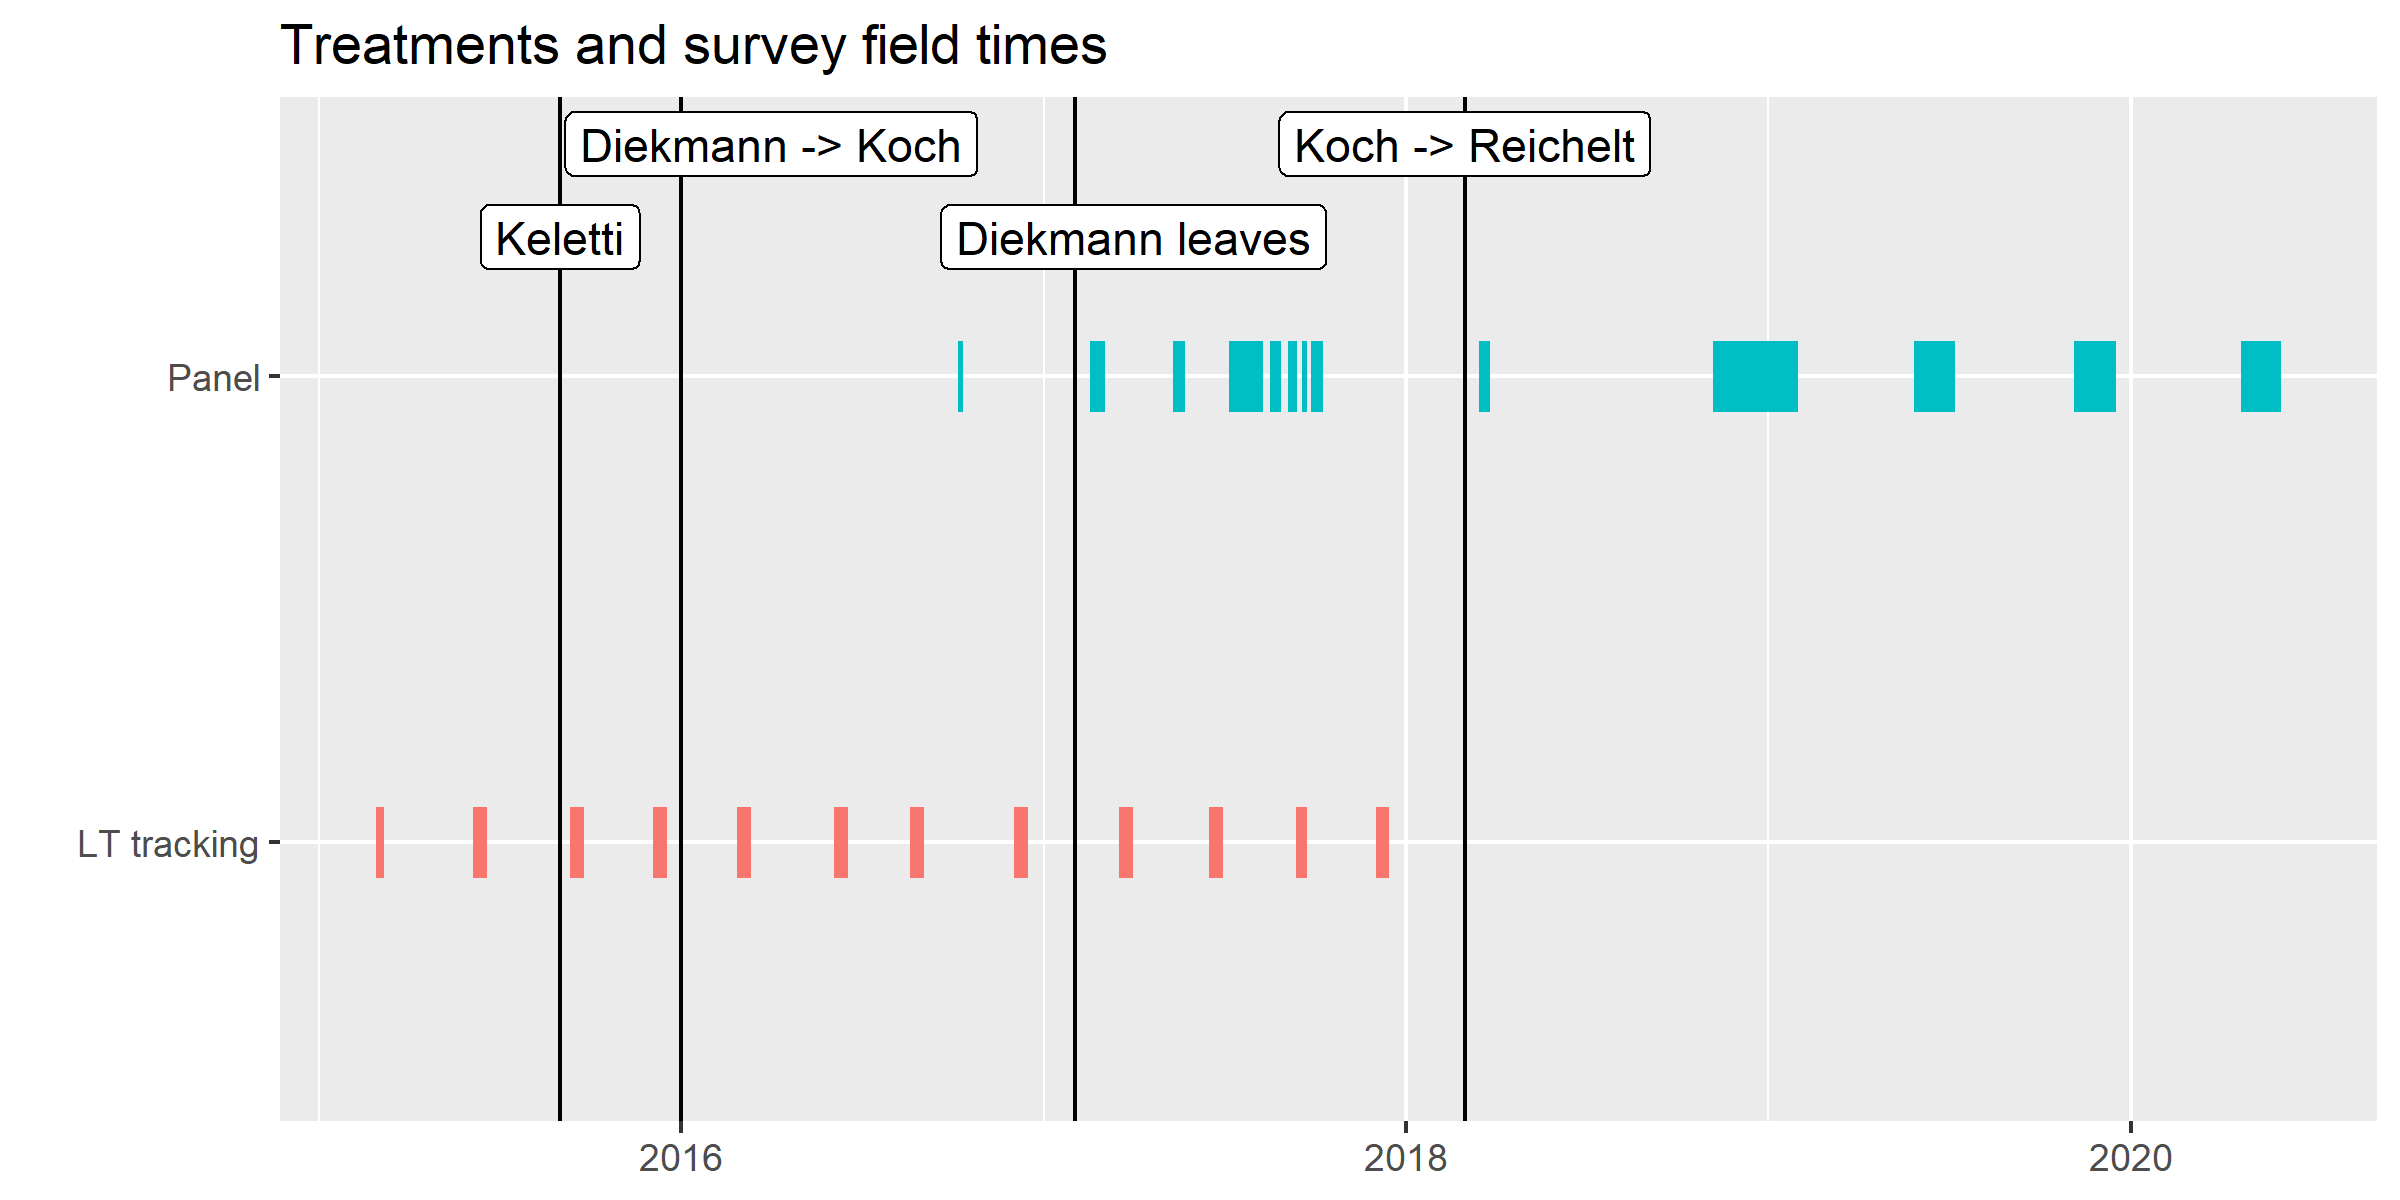
\includegraphics{vis/gles_treatments.png}
\end{frame}

\hypertarget{treatment-selection}{%
\subsection{Treatment selection}\label{treatment-selection}}

\begin{frame}{Treatment selection}
\begin{enumerate}
\item
  Pre-select migration content with supervised classifier.
\item
  Several possible approaches for treatment identification:
\end{enumerate}

\begin{itemize}
\tightlist
\item
  inductive frame identification (FA/STM)
\item
  dictionary for frames (humanitarian/crime/\ldots)
\item
  sentiment towards migration
\end{itemize}

\begin{enumerate}
\setcounter{enumi}{2}
\tightlist
\item
  Treatment identified where parallel paths diverge
\end{enumerate}
\end{frame}

\hypertarget{modelling}{%
\subsection{Modelling}\label{modelling}}

\begin{frame}{Modelling}
Diff-in-Diff:

\center

\[ y = \beta_1 * T + \beta_2 * B + \beta_3 * T * B \]

\begin{itemize}
\tightlist
\item
  DVs: migration attitudes \& issue definitions
\item
  Additional interactions for individual-level moderators.
\end{itemize}
\end{frame}

\hypertarget{measuring-issue-definitions}{%
\subsection{Measuring issue
definitions}\label{measuring-issue-definitions}}

\begin{frame}{Embedding regression (Rodriguez, Spirling, and Stewart
2020)}
\protect\hypertarget{embedding-regression-rodriguez2020}{}
\begin{itemize}
\tightlist
\item
  applicable in low-N environments.
\item
  pre-existing word embeddings to understand how different groups
  communicate about migration.
\item
  assess associations with migration in the MIP answers.
\end{itemize}
\end{frame}

\hypertarget{fin}{%
\subsection{Fin}\label{fin}}

\begin{frame}{Fin}
\center \Large Thank you for your attention!
\end{frame}

\hypertarget{appendix}{%
\section{Appendix}\label{appendix}}

\hypertarget{a-preliminary-effort-at-sentiment-identification}{%
\subsection{A preliminary effort at sentiment
identification}\label{a-preliminary-effort-at-sentiment-identification}}

\begin{frame}[allowframebreaks]{A preliminary effort at sentiment
identification}
\begin{itemize}
\tightlist
\item
  identify sentences mentioning terms from migration dictionary.
\item
  estimate sentiment of these sentences with German BERT sentiment
  classifier (Guhr et al. 2020).
\item
  Trained to classify a variety of German text (wiki, reviews, tweets,
  \ldots) into positive, neutral, and negative content
\end{itemize}

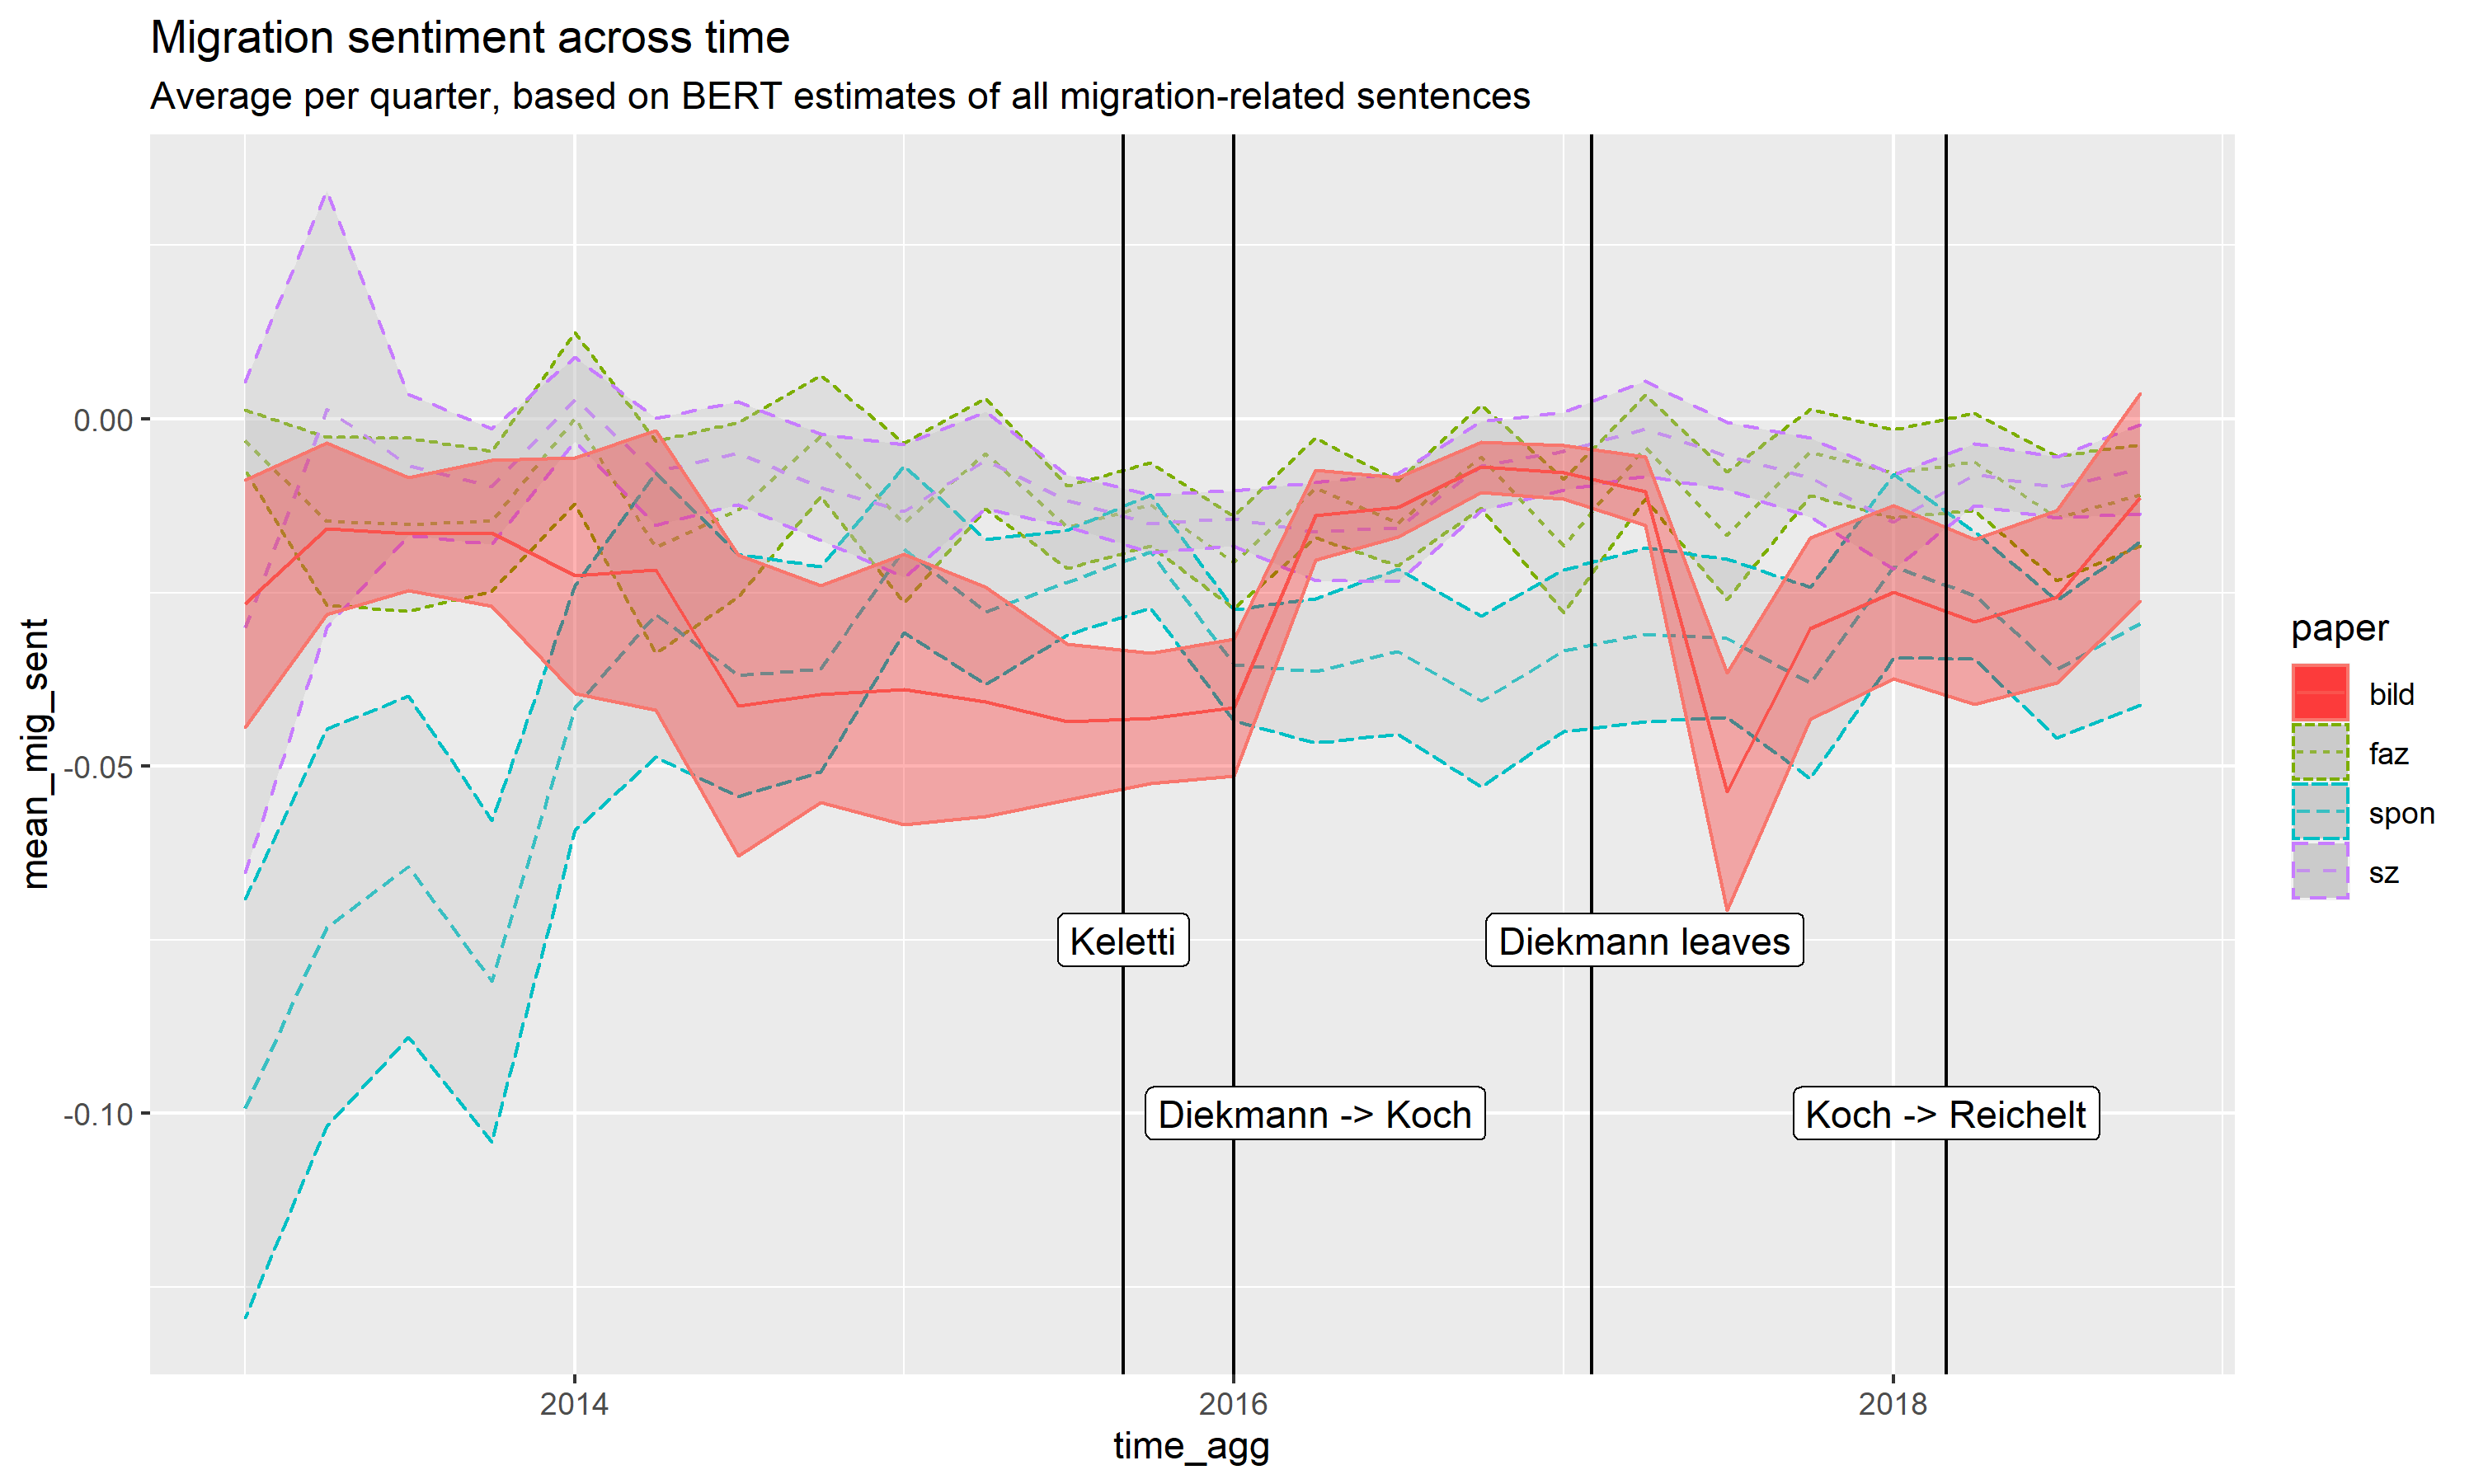
\includegraphics{vis/comparative_sentiment_migration.png}

\framebreak

However, unclear what this really measures:

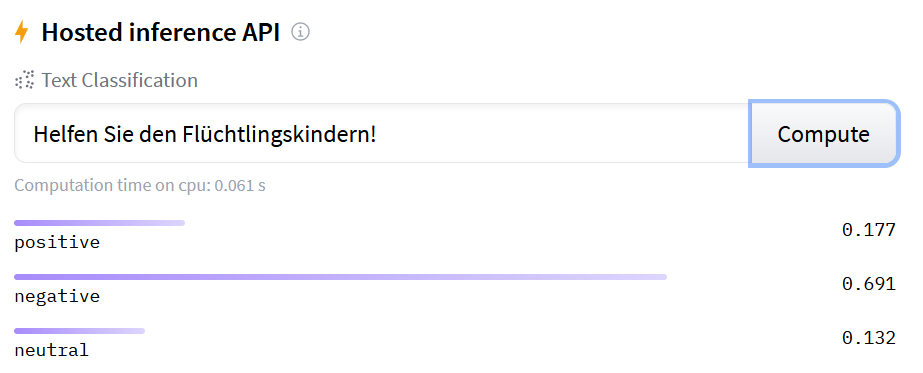
\includegraphics[width=0.45\textwidth,height=\textheight]{vis/BERTProbs2.png}
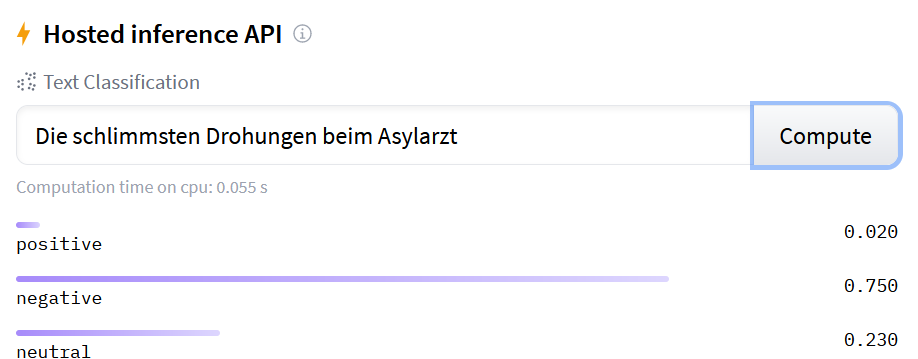
\includegraphics[width=0.45\textwidth,height=\textheight]{vis/BERTProbs3.png}

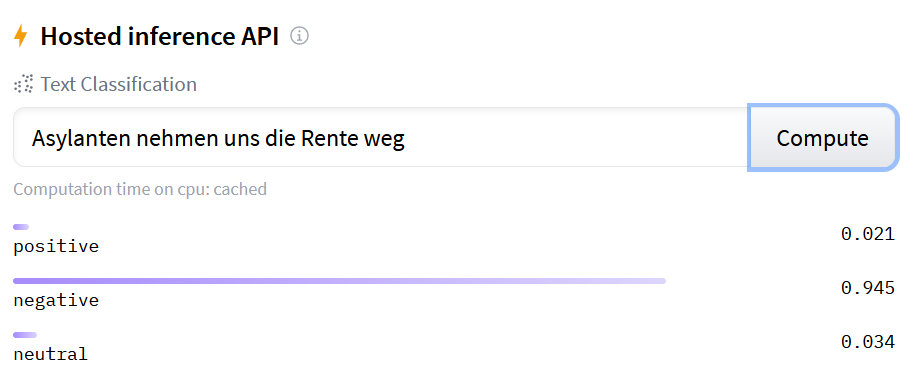
\includegraphics[width=0.45\textwidth,height=\textheight]{vis/BERTProbs4.png}
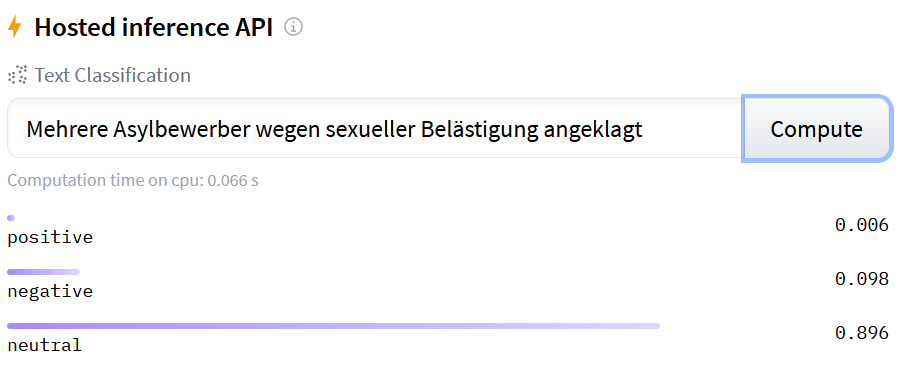
\includegraphics[width=0.45\textwidth,height=\textheight]{vis/BERTProbs5.png}

\framebreak

Takeaways:

\begin{itemize}
\tightlist
\item
  wait for supervised coding.
\item
  focus on specific frames.
\item
  measure association.
\end{itemize}
\end{frame}

\hypertarget{resources}{%
\section{Resources}\label{resources}}

\hypertarget{resources-1}{%
\subsection*{Resources}\label{resources-1}}
\addcontentsline{toc}{subsection}{Resources}

\begin{frame}[allowframebreaks]{Resources}
\hypertarget{refs}{}
\begin{CSLReferences}{1}{0}
\leavevmode\hypertarget{ref-Ajzen2000}{}%
Ajzen, Icek, and Martin Fishbein. 2000. {``{Attitudes and the
Attitude-Behavior Relation: Reasoned and Automatic Processes}.''}
\emph{European Review of Social Psychology} 11 (1): 1--33.
\url{https://doi.org/10.1080/14792779943000116}.

\leavevmode\hypertarget{ref-Bennett2008}{}%
Bennett, W. Lance, and Shanto Iyengar. 2008. {``{A new era of minimal
effects? The changing foundations of political communication}.''}
\emph{Journal of Communication} 58 (4): 707--31.
\url{https://doi.org/10.1111/j.1460-2466.2008.00410.x}.

\leavevmode\hypertarget{ref-Boomgaarden2009}{}%
Boomgaarden, Hajo G., and Rens Vliegenthart. 2009. {``{How news content
influences anti-immigration attitudes: Germany, 1993-2005}.''}
\emph{European Journal of Political Research} 48 (4): 516--42.
\url{https://doi.org/10.1111/j.1475-6765.2009.01831.x}.

\leavevmode\hypertarget{ref-Chiang2011a}{}%
Chiang, Chun Fang, and Brian Knight. 2011. {``{Media bias and influence:
Evidence from newspaper endorsements}.''} \emph{Review of Economic
Studies} 78 (3): 795--820. \url{https://doi.org/10.1093/restud/rdq037}.

\leavevmode\hypertarget{ref-Converse1962}{}%
Converse, Philip E. 1962. {``{Information flow and the stability of
partisan attitudes}.''} \emph{Public Opinion Quarterly} 26 (4): 578--99.
\url{https://doi.org/10.1086/267129}.

\leavevmode\hypertarget{ref-Devine2020}{}%
Devine, Daniel, and Justin Murphy. 2020. {``{Does Media Coverage Drive
Public Support for UKIP or Does Public Support for UKIP Drive Media
Coverage?}''} \emph{British Journal of Political Science} 50 (3):
893--910. \url{https://doi.org/10.1017/S0007123418000145}.

\leavevmode\hypertarget{ref-Foos2020}{}%
Foos, Florian, and Daniel Bischof. 2020. {``{Can the tabloid media
create Eurosceptic attitudes? A quasi-experiment on media innuence in
England},''} no. page 26.

\leavevmode\hypertarget{ref-Gentzkow2011}{}%
Gentzkow, Matthew, Jesse M. Shapiro, and Michael Sinkinson. 2011.
{``{The effect of newspaper entry and exit on electoral politics}.''}
\emph{American Economic Review} 101 (7): 2980--3018.
\url{https://doi.org/10.1257/aer.101.7.2980}.

\leavevmode\hypertarget{ref-Guess2021}{}%
Guess, Andrew M, Pablo Barberá, Simon Munzert, and Junghwan Yang. 2021.
{``{The consequences of online partisan media},''} 1--8.
\url{https://doi.org/10.1073/pnas.2013464118/-/DCSupplemental.y}.

\leavevmode\hypertarget{ref-Guhr2020}{}%
Guhr, Oliver, Anne Kathrin Schumann, Frank Bahrmann, and Hans Joachim
Böhme. 2020. {``{Training a broad-coverage German sentiment
classification model for dialog systems}.''} \emph{LREC 2020 - 12th
International Conference on Language Resources and Evaluation,
Conference Proceedings}, no. May: 1627--32.

\leavevmode\hypertarget{ref-King2017}{}%
King, Gary, Benjamin Schneer, and Ariel White. 2017. {``{How the news
media activate public expression and influence national agendas}.''}
\emph{Science} 358 (November): 776--80.
\url{https://doi.org/10.1007/978-1-349-11336-1_13}.

\leavevmode\hypertarget{ref-Ladd2009a}{}%
Ladd, Jonathan Mc Donald, and Gabriel S. Lenz. 2009. {``{Exploiting a
rare communication shift to document the persuasive power of the news
media}.''} \emph{American Journal of Political Science} 53 (2):
394--410. \url{https://doi.org/10.1111/j.1540-5907.2009.00377.x}.

\leavevmode\hypertarget{ref-Lau2021}{}%
Lau, Richard R., Kathleen Rogers, and Jamel Love. 2021. {``{Media
Effects in the Viewer's Choice Era: Testing Revised Agenda-Setting and
Priming Hypotheses}.''} \emph{Political Communication} 38 (3): 199--221.
\url{https://doi.org/10.1080/10584609.2020.1763526}.

\leavevmode\hypertarget{ref-McCombs1972}{}%
McCombs, Maxwell E., and Donald L Shaw. 1972. {``{The agenda-setting
function of mass media}.''} \emph{Public Opinion Quarterly} 36 (2):
176--87.

\leavevmode\hypertarget{ref-Nelson1997}{}%
Nelson, Thomas E, Rosalee A Clawson, and Zoe Oxley. 1997. {``{Media
Framing of a Civil Liberties Conflict and Its Effect on Tolerance}.''}
\emph{American Political Science Review} 91 (3): 567--83.

\leavevmode\hypertarget{ref-Rodriguez2020}{}%
Rodriguez, Pedro L., Arthur Spirling, and Brandon M. Stewart. 2020.
{``{Embedding Regression: Models for Context-Specific Description and
Inference in Political Science}.''}

\leavevmode\hypertarget{ref-Spirig2020}{}%
Spirig, Judith. 2020. {``{Media Take-Over and Voting Behavior : Can
Politician-Owned Newspapers Sway Voters ?}''}

\leavevmode\hypertarget{ref-Taber2006}{}%
Taber, Charles S, and Milton Lodge. 2006. {``{Motivated Skepticism in
the Evaluation of Political Beliefs}.''} \emph{American Journal of
Political Science} 50 (3): 755--69.

\leavevmode\hypertarget{ref-Zaller1992}{}%
Zaller, John. 1992. \emph{{The nature and origins of mass opinion}}.
Cambridge University Press.

\end{CSLReferences}
\end{frame}

\end{document}
